\section{Best Practice Evaluation}
\label{theory:best-practice}
Since the release of both the Oculus rift\footnote{https://www.oculus.com/rift/} and HTC Vive\footnote{https://www.vive.com/eu/product/} which both have 6 Degrees Of Freedom (DOF) controllers, the number of applications focusing on complex interactions and manipulation has really exploded\footnote{https://www3.oculus.com/en-us/blog/gear-vr-ecosystem-expands-to-include-facebook-360-photos-over-250-apps-and-new-video-content/}. Regular web applications aswell as HTC Vive applications that manipulates 3D objects in a 3D environment was analyzed and evaluated, from with greater insights in popular usage and implementations was gathered.
\subsection{Storyboard VR}
The creative team at Artefact \footnote{https://www.artefactgroup.com/} created a prototyping tool for VR called Storyboard VR \footnote{https://www.artefactgroup.com/work/storyboard-vr/}. This tool gives the user the option to create high fidelity(see section \ref{method:prototype:hifi})  VR prototypes while immerged with a HMD. Objects in the scene are uploaded as high-resolution images and placed in the VE. The essential interactions of this system are explained in this section.
\subsubsection{Tools}
To interact with this system the primary controller is equipped with a ray-casting technique (see section \ref{theory:toolsandtech:raycast}) for selection within the VE.
Most tools in this system can be found on a swipe-based menu, attached to the secondary controller\ref{fig:storyboard}. There are some object-specific selectors (see section \ref{theory:toolsandtech:selector}) attached to each object, these are visible when the object is selected by the user. It is not possible to teleport or in other ways travel in the application, but there are  a timeline/storyline where different 'frames' can be accessed.

\begin{figure}
\begin{subfigure}{.5\textwidth}
  \centering
  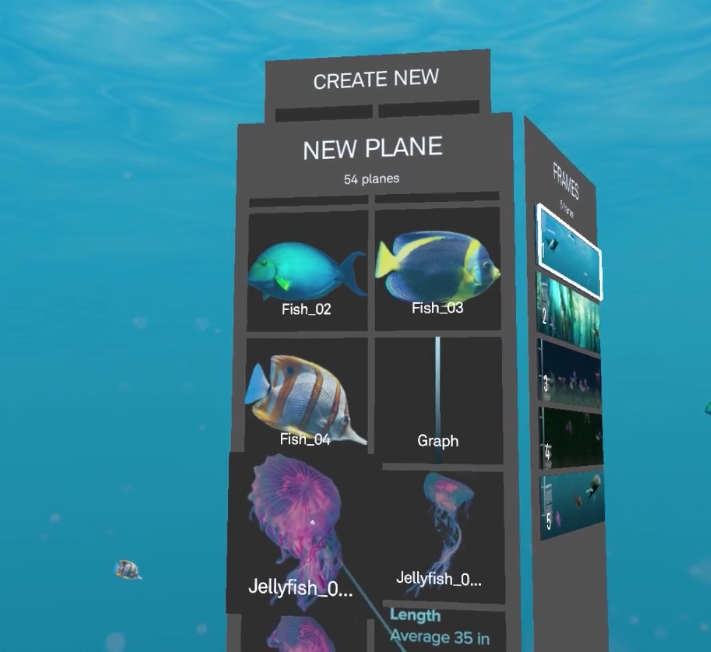
\includegraphics[width=.8\linewidth]{storyboardvr_fishmenu.PNG}
  \caption{Menu for selecting a new object}
  \label{fig:storyboard:fishmenu}
\end{subfigure}%
\begin{subfigure}{.5\textwidth}
  \centering
  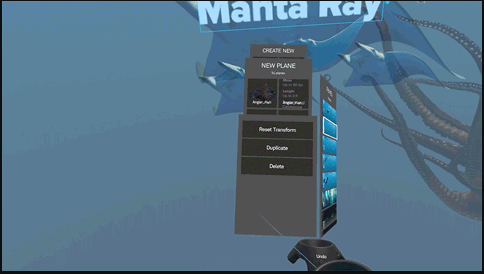
\includegraphics[width=.8\linewidth]{storyboardvr_menu.PNG}
  \caption{Submenu for manipulating a selected object}
  \label{fig:storyboard:menu}
\end{subfigure}
\caption{Menu interfaces in Storyboar VR}
\label{fig:storyboard}
\end{figure}

\begin{itemize}
\item \textbf{Creating objects}
In order to create an object within the world, the user can select from imported images or default 3D shapes from the 'Create' part of the menu. An object that has been created can later be duplicated by selecting 'Duplicate' on the same menu and then selecting the object\ref{fig:storyboard:fishmenu}.
\item \textbf{Selecting and deleting objects}
Objects are selected by pointing the ray from the primary controller on the and clicking the trigger. An object is deleted by selecting the object and selecting remove on the menu\ref{fig:storyboard:menu}.
\item \textbf{Scale and positioning}
Changing the position of an object is achieved by pointing the ray at the object, holding the trigger while moving it into position with the ray, then releasing the trigger. The scale of an object is manipulated by  swiping up or down on the touchpad on top of the primary controller.
\end{itemize}
\subsection{Tilt Brush}
\label{theory:best-practice:tiltbrush}
 One of the applications that was released with HTC Vive is the praised application\footnote{http://store.steampowered.com/app/327140/?l=english} 'Tilt Brush' by Google \footnote{https://www.tiltbrush.com/} where the user can use the existing handcontrollers as paintbrushes and paint in 3D space. This application highlights many of the interactions that are essential when manipulating a VE. Some of these interactions are explained further in this section.
 \begin{itemize}
\item \textbf{Creating objects}
Creating a new painting stroke is the core of the application, and can as such be accessed directly with primary triggers on both controllers.
\item \textbf{Selecting and deleting objects}
Strokes are targeted by placing a spherical tool (attached to your brush) around the stroke and pressing the same trigger that is used for drawing. The tool is activated by selection on the secondary brush menu.
\item \textbf{Parameters and setting}
Tilt Brush mimics the way that painters paint in many ways, most prominent when selecting and changing parameters. The primary controller acts like a paint brushm and the secondary controller acts as a painters palette. The most common and most used tools for what will be painted ( brush-size, undo, deleting strokes etc) are accessed through the primary brush (controller). More complex modifications (brush type, colors etc) are accessed from the secondary brush by activating a menu connected to that brush (controller) and selecting with the other brush.
\item \textbf{Scale and positioning}
One of the biggest advantages of working in a VE is that you are not bound to the restrictions of your physical relationship to the objects that you are working with. By using both controllers and moving them away from each other, the environment grows and the users scale decreases. The user scale can be enlarged by moving the controllers closer together.
By using a raycast (see Section \ref{theory:toolsandtech}) the user can teleport around in the VE.
 \end{itemize}
 \begin{figure}
 \begin{subfigure}{.5\textwidth}
   \centering
   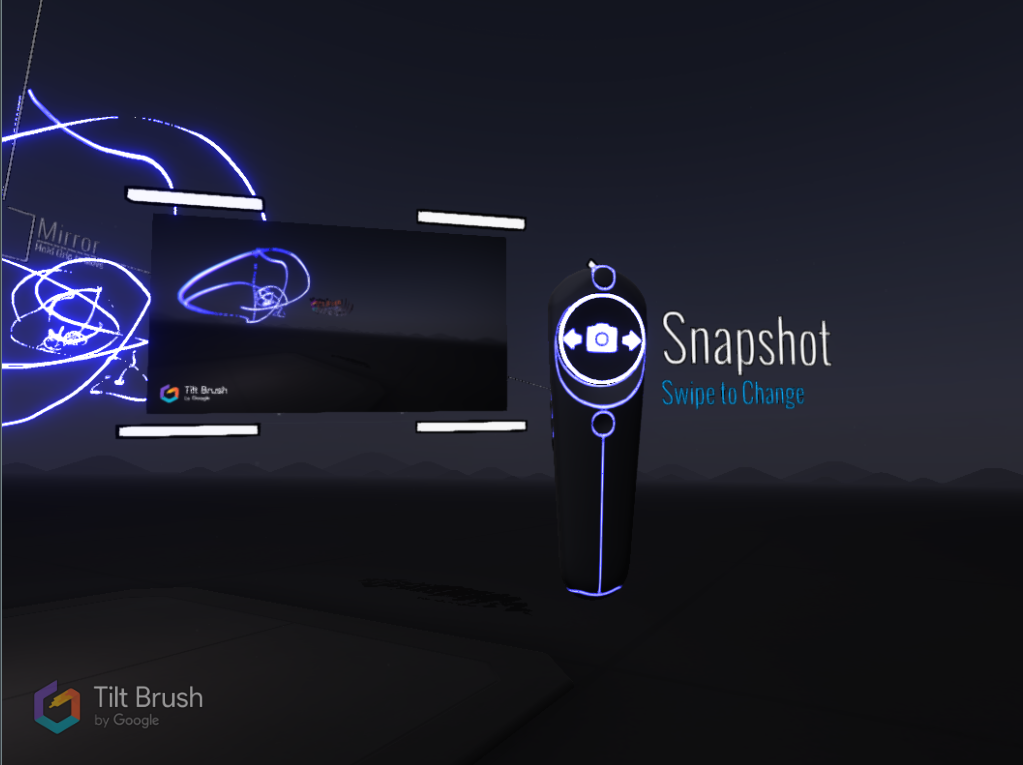
\includegraphics[width=.8\linewidth]{tilt_activemenu.PNG}
   \caption{Active menu. Selection of mode depending on current tool}
   \label{fig:tilt:activemenu}
 \end{subfigure}%
 \begin{subfigure}{.5\textwidth}
   \centering
   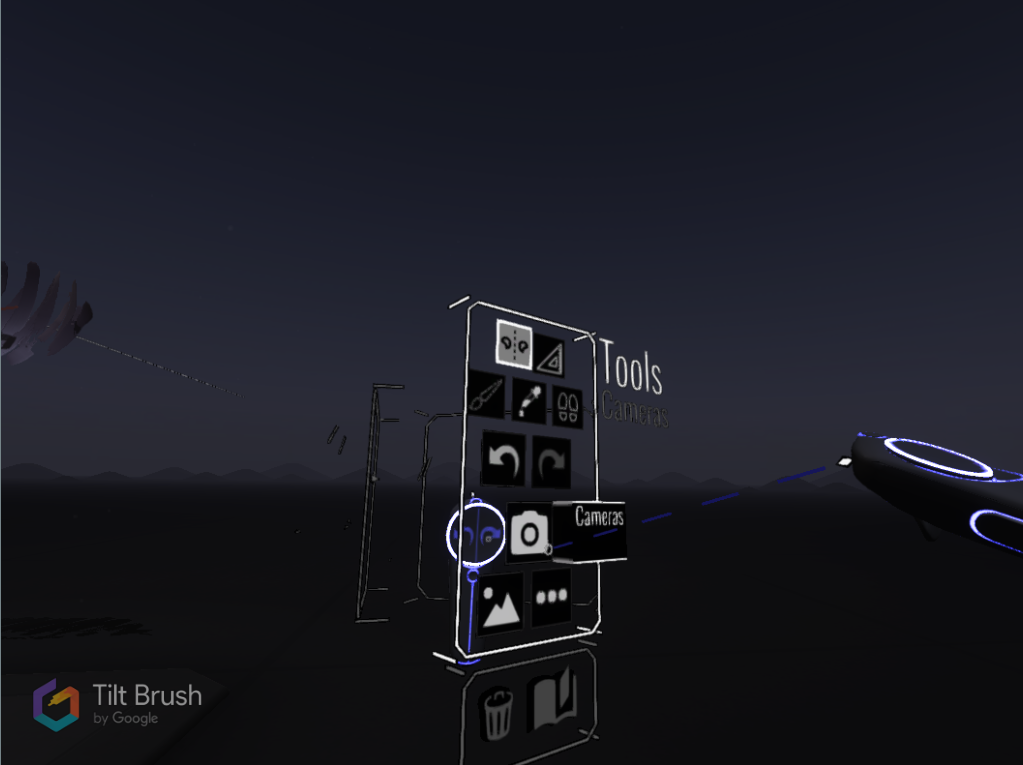
\includegraphics[width=.8\linewidth]{tilt_passivemenu.PNG}
   \caption{Passive menu with all actions and tools. Always avaliable in secondary hand. }
   \label{fig:tilt:passivemenu}
 \end{subfigure}
 \caption{Menu interfaces in Tilt Brush}
 \label{fig:tilt}
 \end{figure}
\subsection{Vizor}
Vizor\footnote{https://vizor.io/} is a web-based application that allow the user to create VR experinces and applications in a web-browser. The application is based on WebVR \footnote{https://webvr.info/} and is Object Oriented (OO), where each object in a scene has properties in the form of other objects. Some of these properties (positioning, scale and rotation) can be accessed and edited in "Build" mode (see Figure \ref{fig:vizor:buildmode}) while more complex properties and inner object are accessed through the "Program" mode (see Figure \ref{fig:vizor:programmode}). This approach allows the user to get a holistic view of the entire scene and all objects aswell as their properties and relations to eachother. instead of a list heirarchy with all of the objects, the scene object is the central hub, connected to all objects in it (except for inner objects that are connected through a parent object). One of these connections is shown in Figure \ref{fig:vizor:hierarchycamera}. The approach to divide the process into two parts is also present in the form of objects and patches, these are displayed in a list (Figure \ref{fig:vizor:objectspatches}). Objects are regular 3D objects that can be added to the scene, patches are properties that can be added to these objects.

\begin{figure}
\begin{subfigure}{.5\textwidth}
  \centering
  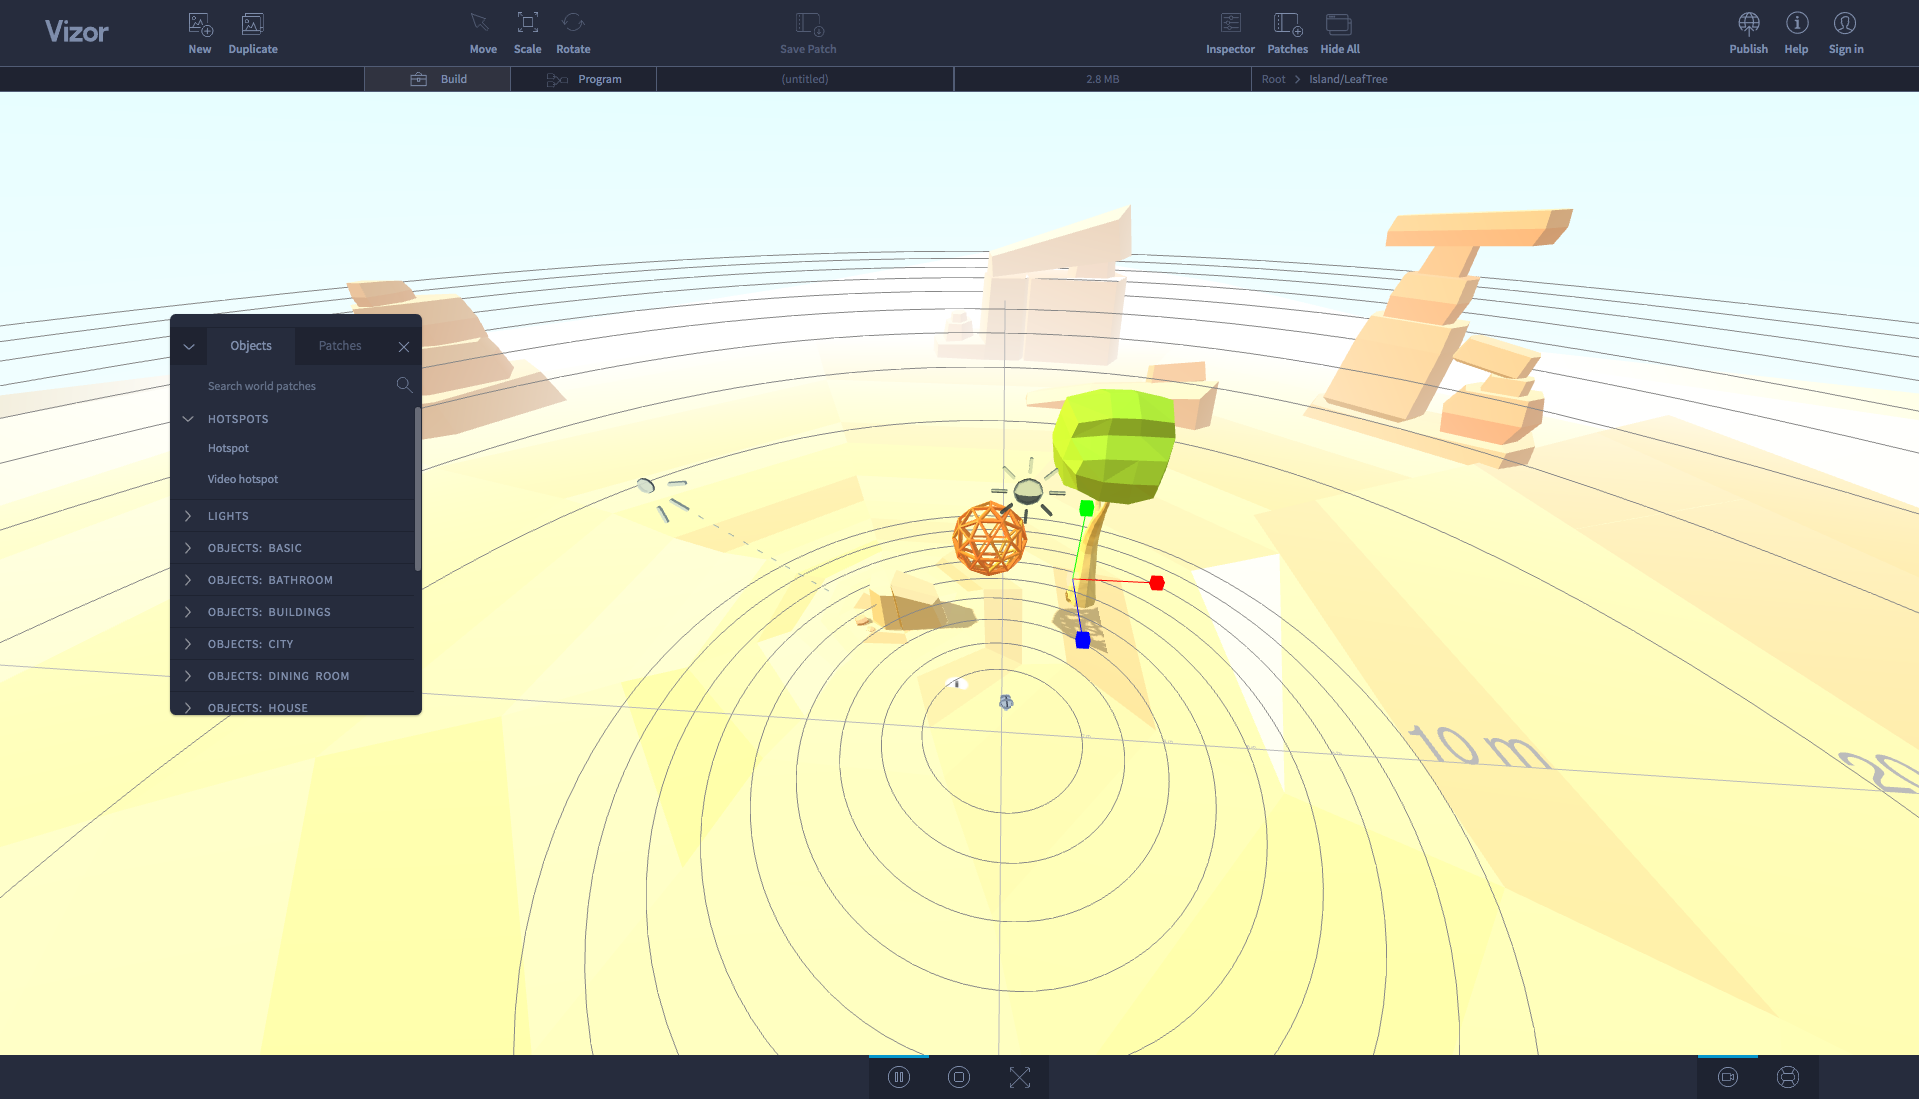
\includegraphics[width=.8\linewidth]{vizor_objects.png}
  \caption{Build mode. Objects can be positioned and scaled with mouse actions.}
  \label{fig:vizor:buildmode}
\end{subfigure}%
\begin{subfigure}{.5\textwidth}
  \centering
  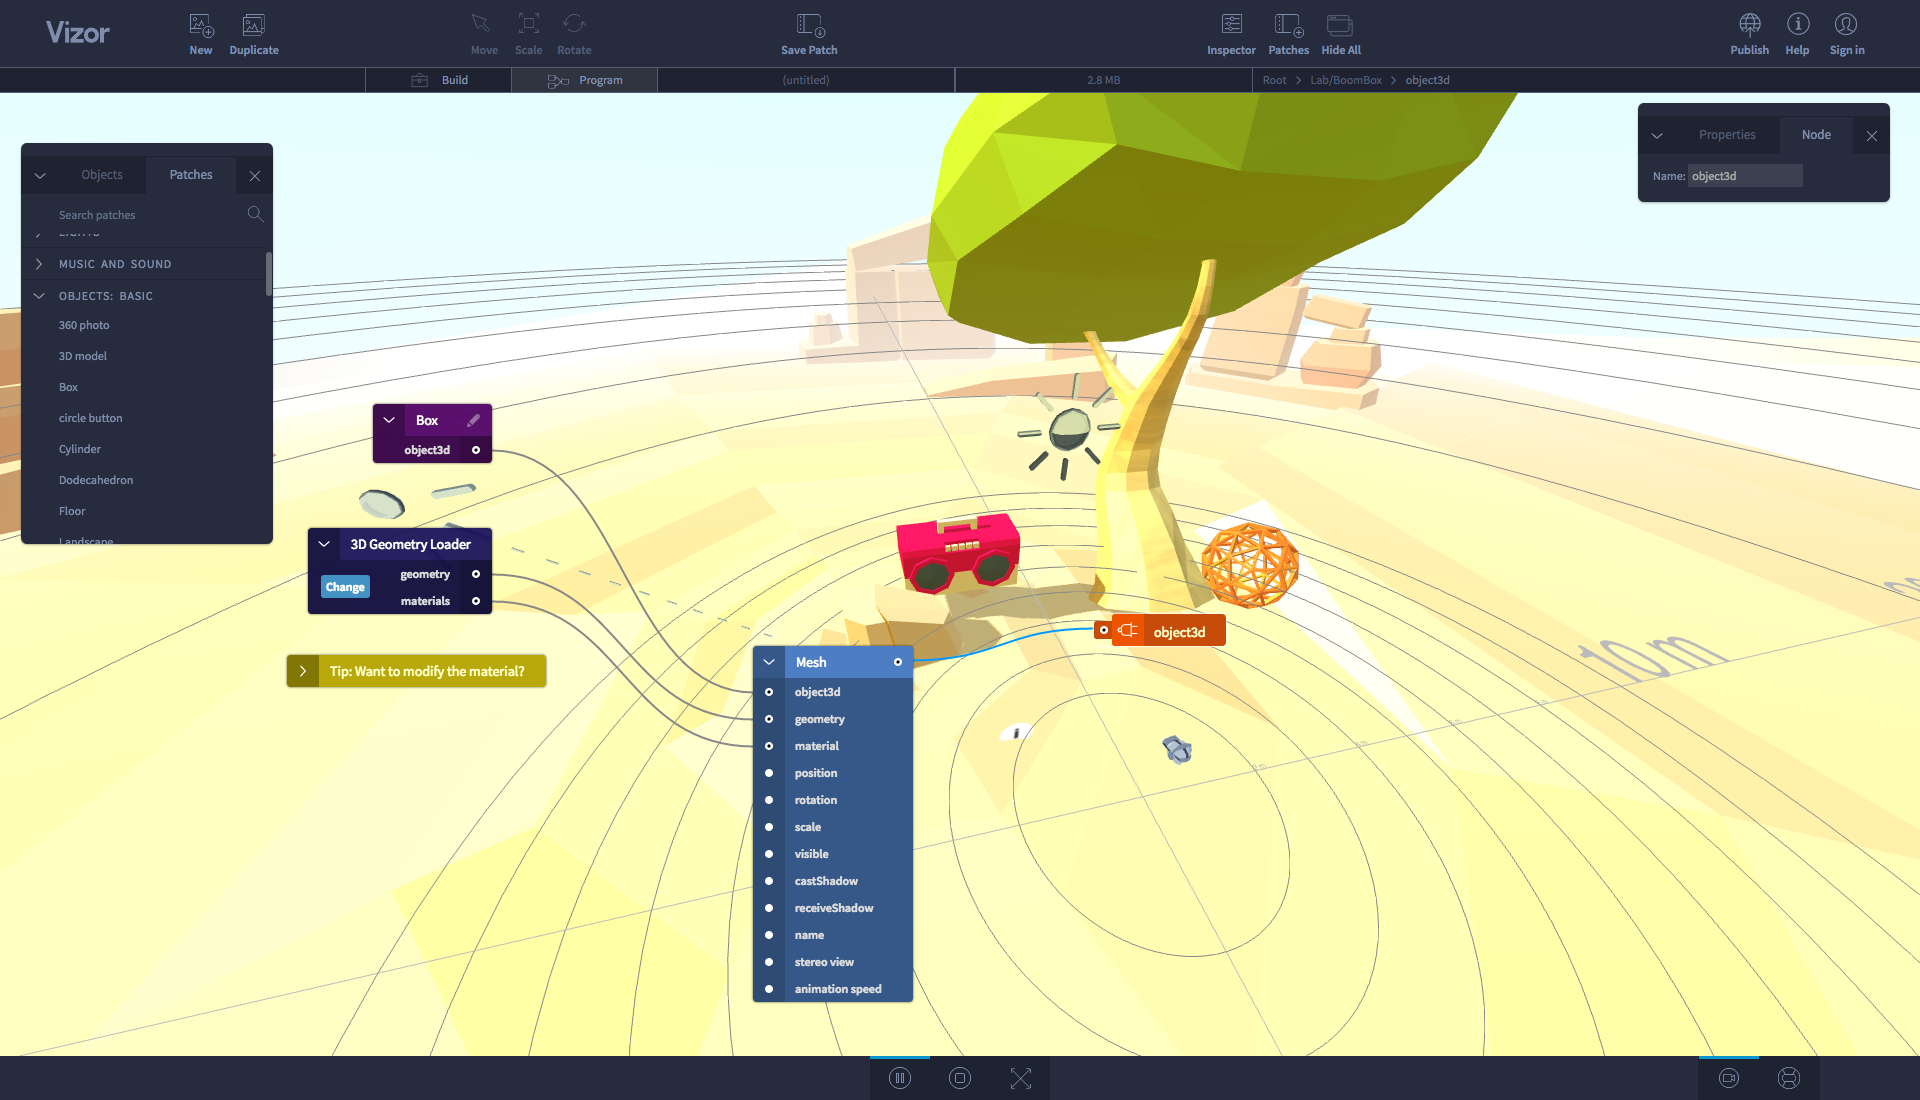
\includegraphics[width=.8\linewidth]{vizor_programming.png}
  \caption{Program mode. Properties and objects can be connected and edited using mouse. }
  \label{fig:vizor:programmode}
\end{subfigure}
\caption{Different modes of web application Vizor}
\label{fig:vizor}
\end{figure}

\begin{figure}
\begin{subfigure}{.5\textwidth}
  \centering
  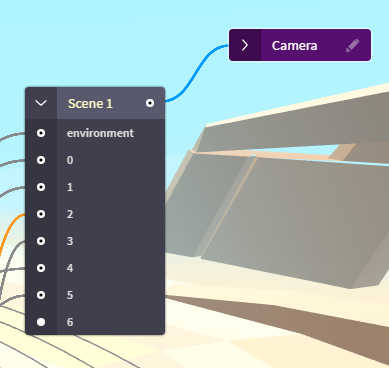
\includegraphics[width=.8\linewidth]{vizor_hierarchy_camera.png}
  \caption{A connection between the scene and the main camera}
  \label{fig:vizor:hierarchycamera}
\end{subfigure}%
\begin{subfigure}{.5\textwidth}
  \centering
  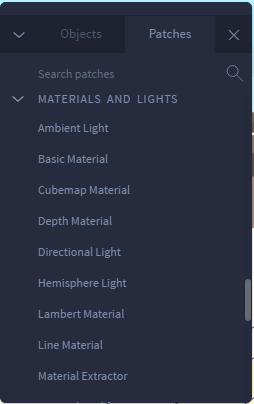
\includegraphics[width=.8\linewidth]{vizor_objects_patches.png}
  \caption{Program mode. Properties and objects can be connected and edited using mouse. }
  \label{fig:vizor:objectspatches}
\end{subfigure}
\caption{Different elements in Vizor}
\label{fig:vizorelements}
\end{figure}
